\documentclass[11pt]{article}

\usepackage[T1]{fontenc}
\usepackage[brazilian]{babel}
\usepackage{graphicx}
\usepackage{geometry}
\usepackage{fancyhdr}
\usepackage{amssymb}
\usepackage{amsmath}
\usepackage{microtype}
\usepackage{url}
\usepackage{booktabs}
\usepackage{tabularx}
\usepackage{hyperref}
\usepackage{xcolor}
\usepackage[round]{natbib}
\usepackage{tikz}
\usetikzlibrary{shapes.geometric, arrows.meta, positioning, calc, fit, backgrounds}

\hypersetup{
    colorlinks=true,
    linkcolor=blue!70!black,
    citecolor=blue!70!black,
    urlcolor=blue!70!black
}

\geometry{
    a4paper,
    width=155mm,
    top=30mm,
    bottom=30mm,
    headheight=56pt,
    headsep=1.2cm,
    bindingoffset=3mm
}

\pagestyle{fancy}
\fancyhead{}

\fancyhead[L]{
    \noindent{\Large \textbf{Ciência de Dados e Inteligência Artificial}}\\
    {\normalsize \textbf{Programa:} Atividade Curricular de Extensão (AEX) -- LABGEP / NIGEP}\\
    {\normalsize \textbf{Orientador:} Prof. Dr. Daniel dos Santos Kaster}
}

\fancyhead[R]{
    
\includegraphics[width=0.38\textwidth]{fig/uel_horizontal.jpg}
}

\renewcommand{\headrulewidth}{0pt}
\fancyheadoffset{1cm}

\begin{document}

\begin{center}
    \Large\textbf{Plano de Projeto: Avaliação, Benchmark e Fine-Tuning de Small Language Models (SLMs) para Automação Orçamentária Pública com n8n}
\end{center}

\medskip

\section*{Identificação do Projeto}

\begin{itemize}
    \item \textbf{Título do Projeto:} Assistente Inteligente para Orçamento Público Estadual baseado em SLMs Locais e Orquestração n8n
    \item \textbf{Instituição / Laboratório:} Universidade Estadual de Londrina (UEL) -- Laboratório de Pesquisa em Gestão Pública (LABGEP / NIGEP)
    \item \textbf{Integrantes (Discentes):} Marcos Vinicius Beregula Ferreira, Guilherme Nascimento Braga
    \item \textbf{Colaboração Técnica:} Rafael Lançoni Santos (Desenvolvimento de Workflows n8n)
    \item \textbf{Coordenação e Orientação:} Prof. Dr. Daniel dos Santos Kaster (Departamento de Computação / UEL)
    \item \textbf{Horizonte de Execução:} Setembro de 2026 a Dezembro de 2026 (Prazo final: 31/12/2026)
\end{itemize}

\section{Contexto, Motivação e Desafio Tecnológico}

No âmbito da gestão governamental, os processos orçamentários do Estado do Paraná são regidos por um arcabouço normativo estrito, sustentado pela Lei Federal n\textordmasculine~4.320/1964 \citep{lei_4320_1964}, pela Lei de Responsabilidade Fiscal (LC n\textordmasculine~101/2000) e por regulamentações estaduais periódicas, destacando-se a Resolução SEFA n\textordmasculine~01/2026 \citep{resolucao_sefa_01_2026} e o Manual Técnico do Orçamento (MTO/PR) \citep{mto_pr_2026}. As rotinas diárias dos servidores públicos envolvem consultas exaustivas a classificadores orçamentários estruturados, tais como:
\begin{itemize}
    \item \textbf{Natureza de Despesa:} Códigos hierárquicos de 6 a 8 dígitos (Categoria Econômica, Grupo, Modalidade de Aplicação, Elemento e Subelemento Detalhe);
    \item \textbf{Ações Orçamentárias:} Atividades, projetos e operações especiais (ex.: Ação 8000 -- Encargos Especiais);
    \item \textbf{Fontes de Recursos:} Identificadores de destinação orçamentária vinculados aos sistemas SIAFIC e MTO;
    \item \textbf{Funções e Subfunções:} Agrupamentos setoriais da despesa pública (ex.: Subfunção 121 -- Planejamento e Orçamento);
    \item \textbf{Dotação Adicional de Despesa (DAD):} Elaboração de justificativas formais técnico-administrativas de esgotamento de alternativas e preservação do equilíbrio orçamentário (Art. 18 da Resolução SEFA 01/2026).
\end{itemize}

Para automatizar o atendimento aos servidores, uma Prova de Conceito (PoC) inicial foi estruturada na plataforma de automação de fluxos \textbf{n8n}. Nos protótipos preliminares disponibilizados pela equipe técnica, o fluxo utiliza nós de agentes inteligentes integrados a ferramentas de consulta em banco relacional PostgreSQL e chamadas a modelos em nuvem (como Google Gemini e Groq/Llama-70B).

Contudo, a transição para um ambiente de produção institucional impõe desafios práticos determinantes:
\begin{enumerate}
    \item \textbf{Mitigação de Custos Financeiros Recorrentes (Modelos Proprietários Pagos):} A dependência de modelos de linguagem comerciais operados em nuvem acarreta custos contínuos e imprevisíveis tarifados por token (além da exigência de contratos em moeda estrangeira), o que compromete a sustentabilidade financeira do serviço público. A adoção de SLMs abertos locais elimina custos de faturamento por uso.
    \item \textbf{Restrição Crítica de Hardware em Produção (Execução Exclusiva em CPU):} O ecossistema de servidores do laboratório e dos órgãos parceiros não dispõe de GPUs dedicadas para processamento de inferência. O assistente deve rodar de forma perene e estável em processadores convencionais (CPU com instruções SIMD como AVX-512 ou ARM NEON).
    \item \textbf{Inadmissibilidade Estrita de Alucinações ($H_{\text{rate}} = 0$):} Em rotinas orçamentárias públicas, códigos inexistentes ou classificações inventadas geram erros fatais em empenhos e liquidações fiscais. As respostas do modelo devem se ater com 100\% de fidelidade aos registros retornados pelas consultas relacionais \citep{ji2023survey}.
    \item \textbf{Segurança, Governança e LGPD (Soberania de Dados):} Embora as leis e dotações orçamentárias sejam de caráter público, normas de governança pública e segurança da informação impedem que dados institucionais, históricos de solicitações e minutas de trabalho sejam trafegados ou armazenados em servidores no exterior sob controle de terceiros.
\end{enumerate}

Para superar esses entraves, este projeto tem como objetivo central \textbf{pesquisar, avaliar mediante benchmarks padronizados e adaptar por Fine-Tuning supervisionado Small Language Models (SLMs) locais e quantizados}, integrando-os de ponta a ponta aos fluxos do n8n.

\section{Fundamentação Teórica e Arquitetura do Sistema}

\subsection{Small Language Models (SLMs) e Leis de Escala}
Historicamente, o paradigma de modelos fundacionais priorizou modelos massivos (de dezenas a centenas de bilhões de parâmetros) baseados na arquitetura Transformer decodificadora \citep{vaswani2017attention}. No entanto, as leis de escala computacionalmente ótimas demonstradas no estudo \textit{Chinchilla} \citep{hoffmann2022training} evidenciaram que modelos de menor porte, quando expostos a conjuntos de dados substancialmente maiores e com alta densidade sintética (de 2 a 15 trilhões de tokens), atingem capacidade de raciocínio, aderência a instruções (\textit{instruction following}) e uso de ferramentas equivalentes ou superiores a modelos massivos de gerações anteriores \citep{allal2024smollm2, yang2024qwen25}.

\subsection{Mecânica da Quantização e Inferência em CPU}
Em modelos de linguagem, os parâmetros são originalmente representados em ponto flutuante de 16 bits (FP16 ou BF16), demandando aproximadamente 2 bytes por parâmetro. Para viabilizar a execução em CPU comum, emprega-se a \textbf{Quantização Pós-Treinamento (PTQ)} baseada no ecossistema GGUF/\texttt{llama.cpp} \citep{gerganov2023llamacpp}:
\begin{itemize}
    \item \textbf{Quantização por Blocos (\textit{k-quants}):} No esquema \texttt{Q4\_K\_M}, os tensores de peso são particionados em superblocos com fatores de escala diferenciados, mantendo as camadas críticas de atenção (\textit{attention layers}) em precisões intermediárias (5 e 6 bits) e as camadas lineares densas em 4 bits, minimizando a perda de perplexidade \citep{dettmers2022llmint8}.
    \item \textbf{Gargalo de Largura de Banda de Memória (\textit{Memory Bandwidth Bound}):} A fase de decodificação autoregressiva em CPU é limitada pela velocidade com que os pesos trafegam da memória RAM principal para os caches L1/L2/L3 do processador \citep{kim2023memory}. Modelos quantizados reduzem o volume de tráfego por um fator de até $4\times$, aumentando substancialmente o throughput em tokens por segundo sem demandar aceleração de tensores em GPU.
\end{itemize}

\subsection{Fundamentos Matemáticos da Adaptação de Baixo Posto (LoRA e QLoRA)}
O Fine-Tuning completo de todos os pesos de uma rede ($\Theta$) em CPU é proibitivo computacionalmente. Adota-se, portanto, a técnica de \textit{Low-Rank Adaptation} (LoRA) \citep{hu2022lora}, que congela a matriz de pesos pré-treinada $W_0 \in \mathbb{R}^{d \times k}$ e injeta matrizes de decomposição de baixo posto:
\begin{equation}
    W = W_0 + \Delta W = W_0 + \frac{\alpha}{r} (B \cdot A)
    \label{eq:lora}
\end{equation}
onde $A \in \mathbb{R}^{r \times k}$ é inicializada por uma distribuição Gaussiana $\mathcal{N}(0, \sigma^2)$, $B \in \mathbb{R}^{d \times r}$ é inicializada em zero, $r \ll \min(d, k)$ representa o posto intrínseco de adaptação (tipicamente $r \in \{8, 16, 32\}$) e $\alpha$ é o hiperparâmetro de escala. 

O método QLoRA \citep{dettmers2023qlora} estende essa formulação aplicando o tipo de dados 4-bit \textit{NormalFloat} (NF4), quantização dupla (\textit{Double Quantization} -- DQ) e otimizadores paginados (\textit{Paged Optimizers}), reduzindo drasticamente o consumo de memória na fase de treinamento. Concluído o ajuste, os adaptadores $\Delta W$ são fundidos diretamente em $W_0$ (\textit{weight merging}), permitindo a exportação para o formato GGUF sem introduzir qualquer sobrecarga computacional (\textit{overhead}) de latência na inferência final.

\subsection{Arquitetura Geral Integrada}
A Figura~\ref{fig:arquitetura} ilustra o fluxo operacional concebido. As consultas são recebidas por webhooks do n8n, processadas por nós de memória e roteadas aos subagentes. O SLM local realiza o parsing e a extração determinística de entidades e radicais, que alimentam as ferramentas SQL conectadas ao PostgreSQL. As respostas consolidadas são devolvidas ao servidor público em JSON parseável ou Markdown higienizado.

\begin{figure}[ht!]
\centering
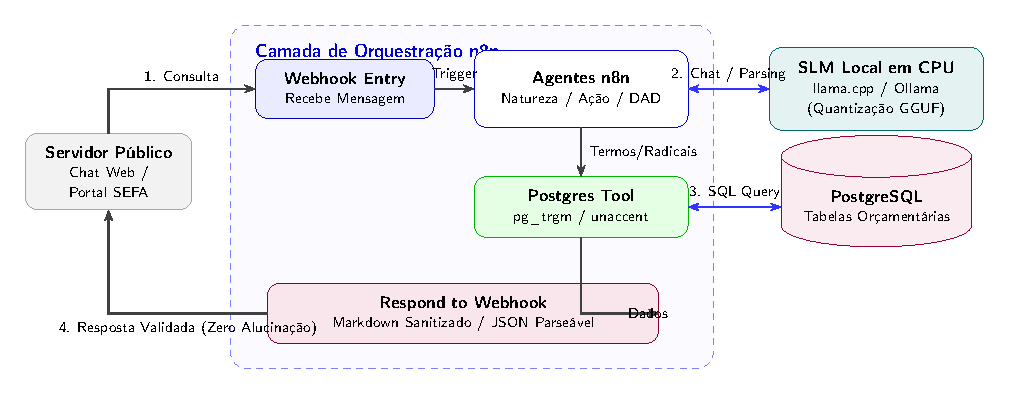
\includegraphics[width=\textwidth]{fig/fig}
\caption{Visão Geral da Arquitetura Integrada: Usuário, Camada de Orquestração n8n, SLM Local em CPU e PostgreSQL.}
\label{fig:arquitetura}
\end{figure}

O diagrama completo da solução foi estruturado no formato nativo do Draw.io, localizado em \path{docs/diagramas/fig.drawio}, permitindo customizações visuais e exportação direta para a pasta de figuras (\path{docs/fig/fig.pdf}).

\section{Metodologia Experimental e Roteiro de Execução}

O projeto está delineado em quatro etapas metodológicas rigorosas, detalhadas a seguir de modo a fornecer uma referência técnica clara para implementação e replicação.

\subsection{Etapa 1: Pesquisa Sistemática e Triagem dos Modelos Candidatos}
Seguindo as diretrizes acadêmicas formuladas pelo Prof. Daniel Kaster, serão selecionados modelos representativos da literatura atual em duas classes de operação:

\begin{enumerate}
    \item \textbf{Classe A -- Modelos Ultraleves (1B a 3B):} Projetados para execução instantânea em CPU com baixa ocupação de memória RAM ($< 3{,}5\text{ GB}$). Atuarão na triagem de mensagens, classificação de intenção (saudação vs. consulta direta) e extração determinística de entidades léxicas para chamadas de ferramentas (\textit{tool calling}) \citep{schick2023toolformer}. Os principais expoentes incluem o Qwen 2.5 1.5B/3B \citep{yang2024qwen25}, Llama 3.2 1B/3B \citep{dubey2024llama3} e SmolLM2 1.7B \citep{allal2024smollm2}.
    \item \textbf{Classe B -- Modelos Intermediários de Alta Capacidade (3.8B a 8B):} Focados em tarefas cognitivas complexas, como interpretação de dispositivos legais do MTO-PR, resolução de ambiguidades orçamentárias e síntese de minutas de DAD em JSON estrito sem desvios gramaticais \citep{willard2023efficient}. Destacam-se as famílias Phi-3.5/Phi-4-mini \citep{abdin2024phi3}, Gemma 2 \citep{gemmateam2024gemma2}, Qwen 2.5 7B \citep{yang2024qwen25} e Llama 3.1 8B \citep{dubey2024llama3}.
\end{enumerate}

\begin{table}[ht!]
\centering
\small
\setlength{\tabcolsep}{5pt}
\renewcommand{\arraystretch}{1.25}
\caption{Matriz Comparativa dos SLMs Candidatos para Benchmark em CPU (quantização padrão GGUF Q4\_K\_M).}
\label{tab:candidatos_slm}
\begin{tabularx}{\textwidth}{>{\bfseries}p{3.2cm} c c c c >{\raggedright\arraybackslash}X}
\toprule
\textbf{Modelo} & \textbf{Tamanho} & \textbf{Contexto} & \textbf{Quant.} & \textbf{RAM} & \textbf{Papel no Sistema / Atribuição} \\
\midrule
\multicolumn{6}{@{}l}{\textit{\textbf{Classe A: Modelos Ultraleves ($< 3{,}5$ GB RAM) -- Triagem e Tool Calling}}} \\[2pt]
Qwen 2.5 1.5B & 1{,}5B & 32k & Q4\_K\_M & $\sim$ 1{,}4 GB & Extração determinística e parsing rápido \\
Llama 3.2 1B & 1{,}2B & 128k & Q4\_K\_M & $\sim$ 1{,}2 GB & Classificação de intenção e saudação \\
SmolLM2 1.7B & 1{,}7B & 8k & Q4\_K\_M & $\sim$ 1{,}5 GB & Extração de parâmetros e radicais \\
Qwen 2.5 3B & 3{,}1B & 32k & Q4\_K\_M & $\sim$ 2{,}6 GB & Tool calling estruturado e fallback \\
Llama 3.2 3B & 3{,}2B & 128k & Q4\_K\_M & $\sim$ 2{,}8 GB & Parsing semântico e roteamento \\
\midrule
\multicolumn{6}{@{}l}{\textit{\textbf{Classe B: Modelos Intermediários -- Raciocínio MTO e Minutas DAD}}} \\[2pt]
Phi-3.5-mini & 3{,}8B & 128k & Q4\_K\_M & $\sim$ 3{,}2 GB & Análise de conformidade MTO/PR \\
Phi-4-mini & 3{,}8B & 128k & Q4\_K\_M & $\sim$ 3{,}4 GB & Raciocínio lógico e justificativas fiscais \\
Gemma 2 2.6B & 2{,}6B & 8k & Q4\_K\_M & $\sim$ 2{,}3 GB & Modelo híbrido para síntese concisa \\
Qwen 2.5 7B & 7{,}6B & 128k & Q4\_K\_M & $\sim$ 5{,}8 GB & Síntese avançada de minutas de DAD \\
Llama 3.1 8B & 8{,}0B & 128k & Q4\_K\_M & $\sim$ 6{,}2 GB & Baseline teto comparativo (máxima precisão) \\
\bottomrule
\end{tabularx}
\end{table}

\subsection{Etapa 2: Framework de Benchmarking Empírico em CPU}
A avaliação de desempenho será conduzida por meio de um script automatizado em Python executando testes locais via \texttt{llama.cpp server} e \texttt{Ollama}, alimentado por um conjunto canônico de 100 consultas reais extraídas das interações com o sistema orçamentário.

As métricas mensuradas dividem-se em duas categorias:
\begin{enumerate}
    \item \textbf{Métricas Computacionais de Sistema (CPU Hardware Metrics):}
    \begin{itemize}
        \item \textbf{Throughput de Geração ($T_{\text{gen}}$):} Taxa de tokens por segundo durante a geração autoregressiva com $N \in \{4, 8\}$ threads de CPU:
        \begin{equation}
            T_{\text{gen}} = \frac{N_{\text{tokens}}}{t_{\text{geração}}} \quad [\text{tokens/s}]
        \end{equation}
        \item \textbf{Time-To-First-Token (TTFT):} Intervalo de latência em segundos decorrido entre o envio do prompt com histórico de sessão e a emissão do primeiro token da resposta (avaliação do custo computacional do \textit{prefill} na CPU).
        \item \textbf{Ocupação Máxima de Memória (\textit{Peak RSS RAM}):} Consumo máximo de memória residente em GB aferido via chamadas de sistema (\texttt{getrusage}).
    \end{itemize}
    \item \textbf{Métricas de Qualidade Normativa e Acurácia de Tarefa:}
    \begin{itemize}
        \item \textbf{Acurácia de Triagem de Intenção ($A_{\text{int}}$):} Taxa de acerto binário na classificação de mensagens entre saudações (que devem emitir mensagem padrão imediata sem acionar o banco) e consultas operacionais de despesas.
        \item \textbf{Precisão na Extração de Entidades SQL ($P_{\text{sql}}$):} Conformidade estrita na extração dos três termos (\texttt{termo1}, \texttt{termo2}, \texttt{termo3}) e seus respectivos radicais morfológicos (ex.: conversão para substantivo singular, remoção de acentos diacríticos e isolamento de radicais com 4 a 5 caracteres).
        \item \textbf{Validade Sintática de Saída Estruturada ($V_{\text{json}}$):} Porcentagem de instâncias no fluxo de DAD que produzem objetos JSON válidos sem a presença de caracteres de formatação externos (\textit{markdown fences} ou quebras espúrias).
        \item \textbf{Taxa de Alucinação Orçamentária ($H_{\text{rate}}$):} Frequência de respostas onde o modelo gera códigos numéricos inexistentes ou cria justificativas sem base factual nos dados retornados pela ferramenta \citep{ji2023survey}:
        \begin{equation}
            H_{\text{rate}} = \frac{N_{\text{respostas alucinadas}}}{N_{\text{total de consultas}}} \times 100\% \quad (\text{meta: } 0\%)
        \end{equation}
    \end{itemize}
\end{enumerate}

A partir desses dados, será estabelecido o \textit{ranking} que definirá os dois modelos finais (\textbf{Top-1 Leve} e \textbf{Top-1 Intermediário}).

\subsection{Etapa 3: Curadoria de Dados e Fine-Tuning de Domínio (SFT via QLoRA)}
A literatura demonstra que o ajuste supervisionado (\textit{Supervised Fine-Tuning} -- SFT) é indispensável para incutir o vocabulário e o estilo formal exigidos pela administração pública paranaense, reduzindo drasticamente o tamanho dos prompts do sistema e, por consequência, o tempo de processamento de prefill na CPU.

\begin{enumerate}
    \item \textbf{Construção do Corpus de Ajuste Fino:} Estruturação de um conjunto com aproximadamente $1.500$ pares de instrução-resposta no padrão \texttt{ChatML} ou \texttt{Alpaca}, contemplando:
    \begin{itemize}
        \item O Manual Técnico do Orçamento (MTO) e a classificação orçamentária da despesa pública do Paraná \citep{mto_pr_2026};
        \item O acervo de minutas e despachos da Resolução SEFA 01/2026 \citep{resolucao_sefa_01_2026};
        \item Cenários explícitos de ausência de registros no PostgreSQL, condicionando o modelo a emitir respostas padronizadas de recusa ("\textit{Não encontrei esta despesa no banco de dados}") em vez de inferir códigos inexistentes.
    \end{itemize}
    \item \textbf{Protocolo de Treinamento QLoRA:}
    \begin{itemize}
        \item \textbf{Hiperparâmetros de Adaptação:} Posto $r = 16$, fator de escala $\alpha = 32$ e taxa de descarte (\textit{dropout}) de $0{,}05$, aplicados a todos os módulos lineares de projeção (\texttt{q\_proj}, \texttt{k\_proj}, \texttt{v\_proj}, \texttt{o\_proj}, \texttt{gate\_proj}, \texttt{up\_proj}, \texttt{down\_proj});
        \item \textbf{Otimização:} Otimizador AdamW de 8 bits (\texttt{paged\_adamw\_8bit}), taxa de aprendizado inicial $\eta = 2 \times 10^{-4}$ com decaimento por cosseno (\textit{cosine schedule}) e $3$ épocas completas de treinamento;
        \item \textbf{Fusão e Quantização Final:} Fusão dos pesos $\Delta W$ à matriz base $W_0$ com conversão subsequente via script \texttt{convert\_hf\_to\_gguf.py} para quantização \texttt{Q4\_K\_M}, gerando os artefatos binários finais prontos para implantação em CPU.
    \end{itemize}
\end{enumerate}

\subsection{Etapa 4: Integração Local no n8n e Validação Operacional}
Na etapa final de implantação:
\begin{itemize}
    \item O servidor de inferência local será inicializado como serviço contínuo via \texttt{llama.cpp server} expondo um endpoint HTTP compatível com a API da OpenAI na porta local \texttt{8080};
    \item Os nós de agentes no n8n serão reconfigurados para apontar para o nó \texttt{OpenAI Chat Model} com base URL \url{http://localhost:8080/v1}, com \texttt{temperature} fixada em $0{,}0$ para tarefas determinísticas de extração SQL e $0{,}3$ para redação de DAD;
    \item Serão executados testes de estresse de requisições concorrentes simulando o uso simultâneo por múltiplos técnicos orçamentários.
\end{itemize}

\section{Cronograma e Plano de Ação}

O plano de trabalho está organizado em cinco ciclos quinzenais até o encerramento do período letivo:

\begin{itemize}
    \item \textbf{Ciclo 1 (08/09 a 22/09) -- Preparação de Infraestrutura e Testbed:}
    Configuração do ambiente de execução local em CPU (\texttt{llama.cpp} compilado com flags de vetorização AVX-512 e \texttt{Ollama}). Download e quantização dos candidatos da Tabela~\ref{tab:candidatos_slm}. Construção do script em Python para coleta de métricas e extração do dataset de 100 consultas orçamentárias.
    \textit{Responsáveis: Marcos Beregula e Guilherme Nascimento.}

    \item \textbf{Ciclo 2 (23/09 a 07/10) -- Execução dos Benchmarks e Seleção Top-2:}
    Execução integral da suite de testes de inferência em CPU. Tabulação comparativa de throughput (tokens/s), consumo de RAM, taxa de conformidade JSON e precisão na extração de radicais para PostgreSQL. Reunião de alinhamento com o orientador Prof. Daniel Kaster para ratificação dos modelos eleitos.
    \textit{Responsáveis: Marcos Beregula, Guilherme Nascimento e Prof. Daniel Kaster.}

    \item \textbf{Ciclo 3 (08/10 a 05/11) -- Engenharia de Dados e Fine-Tuning QLoRA:}
    Sistematização dos textos do MTO-PR e Resolução SEFA 01/2026 no formato de instrução supervisionada. Execução do treinamento dos adaptadores QLoRA para o modelo leve e o modelo intermediário. Validação de curvas de perda e fusão dos adaptadores para exportação em GGUF.
    \textit{Responsáveis: Marcos Beregula e Guilherme Nascimento.}

    \item \textbf{Ciclo 4 (06/11 a 30/11) -- Integração de Servidor e Homologação n8n:}
    Conexão dos modelos calibrados aos fluxos do n8n em substituição às APIs externas de nuvem. Realização de testes de validação com os fluxos de Natureza de Despesa, Ação Orçamentária e Minutas DAD.
    \textit{Responsáveis: Toda a equipe (Marcos Beregula, Guilherme Nascimento, Rafael Lançoni e Prof. Daniel Kaster).}

    \item \textbf{Ciclo 5 (01/12 a 20/12) -- Avaliação Final e Relatório de Extensão:}
    Consolidação dos resultados empíricos, redação do relatório final de extensão da UEL e entrega da documentação e repositório de código para os pesquisadores do LABGEP/NIGEP.
    \textit{Responsáveis: Toda a equipe.}
\end{itemize}

\bibliographystyle{apalike}
\bibliography{references}

\end{document}
